\documentclass[12pt]{article}

\usepackage{bm}
\usepackage{amsmath, mathtools}
\usepackage{amsfonts}
\usepackage{amssymb}
\usepackage{graphicx}
\usepackage{colortbl}
\usepackage{xr}
\usepackage{hyperref}
\usepackage{longtable}
\usepackage{xfrac}
\usepackage{tabularx}
\usepackage{float}
\usepackage{siunitx}
\usepackage{booktabs}

%\usepackage{refcheck}

\hypersetup{
    bookmarks=true,         % show bookmarks bar?
      colorlinks=true,       % false: boxed links; true: colored links
linkcolor=red, % color of internal links (change box color with linkbordercolor)
    citecolor=green,        % color of links to bibliography
    filecolor=magenta,      % color of file links
    urlcolor=cyan           % color of external links
}
\newcommand{\NN}[1]{{\color{red}#1}}
\newcommand{\WSS}[1]{{\color{blue}#1}}

\newcommand{\colZwidth}{1.0\textwidth}
\newcommand{\blt}{- } %used for bullets in a list
\newcommand{\colAwidth}{0.13\textwidth}
\newcommand{\colBwidth}{0.82\textwidth}
\newcommand{\colCwidth}{0.1\textwidth}
\newcommand{\colDwidth}{0.05\textwidth}
\newcommand{\colEwidth}{0.8\textwidth}
\newcommand{\colFwidth}{0.17\textwidth}
\newcommand{\colGwidth}{0.5\textwidth}
\newcommand{\colHwidth}{0.28\textwidth}
\newcounter{defnum} %Definition Number
\newcommand{\dthedefnum}{GD\thedefnum}
\newcommand{\dref}[1]{GD\ref{#1}}
\newcounter{datadefnum} %Datadefinition Number
\newcommand{\ddthedatadefnum}{DD\thedatadefnum}
\newcommand{\ddref}[1]{DD\ref{#1}}
\newcounter{theorynum} %Theory Number
\newcommand{\tthetheorynum}{T\thetheorynum}
\newcommand{\tref}[1]{T\ref{#1}}
\newcounter{tablenum} %Table Number
\newcommand{\tbthetablenum}{T\thetablenum}
\newcommand{\tbref}[1]{TB\ref{#1}}
\newcounter{assumpnum} %Assumption Number
\newcommand{\atheassumpnum}{P\theassumpnum}
\newcommand{\aref}[1]{A\ref{#1}}
\newcounter{goalnum} %Goal Number
\newcommand{\gthegoalnum}{P\thegoalnum}
\newcommand{\gsref}[1]{GS\ref{#1}}
\newcounter{instnum} %Instance Number
\newcommand{\itheinstnum}{IM\theinstnum}
\newcommand{\iref}[1]{IM\ref{#1}}
\newcounter{reqnum} %Requirement Number
\newcommand{\rthereqnum}{P\thereqnum}
\newcommand{\rref}[1]{R\ref{#1}}
\newcounter{lcnum} %Likely change number
\newcommand{\lthelcnum}{LC\thelcnum}
\newcommand{\lcref}[1]{LC\ref{#1}}

\newcommand{\tclad}{T_\text{CL}}
\newcommand{\degree}{\ensuremath{^\circ}}
\newcommand{\progname}{SWHS}


%% Comments
\newif\ifcomments\commentstrue

\ifcomments
\newcommand{\authornote}[3]{\textcolor{#1}{[#3 ---#2]}}
\newcommand{\todo}[1]{\textcolor{red}{[TODO: #1]}}
\else
\newcommand{\authornote}[3]{}
\newcommand{\todo}[1]{}
\fi

\newcommand{\wss}[1]{\authornote{magenta}{SS}{#1}}
\newcommand{\nd}[1]{\authornote{blue}{ND}{#1}}
\newcommand{\awh}[1]{\authornote{red}{AD}{#1}}
\usepackage{fullpage}

\begin{document}

\title{Software Requirements Specification for Constraints in Chipmunk2D} 
\author{Alex Halliwushka}
\date{\today}
	
\maketitle

\tableofcontents

%1.2 Table of units
\section{Table of Symbols}

The table that follows summarizes the symbols used in this document along with
their units. The symbols are listed in alphabetical order.

\renewcommand{\arraystretch}{1.2}
%\noindent \begin{tabularx}{1.0\textwidth}{l l X}
\noindent \begin{longtable}{l l p{12cm}} \toprule
  \textbf{symbol} & \textbf{unit} & \textbf{description}\\
  \midrule 
  $\bf b$ & \si[per-mode=symbol]    & Error correction term
  \\ 
  $\beta$ & \si[per-mode=symbol]    & Ratio between two angular velocities
  \\ 
  $e_\text{c}$ & \si[per-mode=symbol]   & Error calculation
  \\ 
$\bf{g_\text{a}}$ & \si[per-mode=symbol] {\kilo\gram\metre^{2}} & Position of
the beginning of the groove
  \\ 
$\bf{g_\text{b}}$ & \si[per-mode=symbol] {\kilo\gram\metre^{2}} & Position of
the end of the groove
  \\ 
$ I_\text{i}$ & \si[per-mode=symbol] {\kilo\gram\metre^{2}} & Moment of inertia
of the ith object
  \\ 
  $\bf{J}$ & \si[per-mode=symbol] {\newton\second}   & Impulse
  \\  
  $\bf{k}$ & \si[per-mode=symbol]    & Mass Matrix
  \\  
  $k_\text{erp}$ & \si[per-mode=symbol]    & Error reduction parameter
  \\  
  $\Delta L$ & \si[per-mode=symbol]   & Change in angular momentum
  \\ 
  $m_\text{i}$ & \si[per-mode=symbol] {\kilo\gram}   & Mass of the ith object
  \\ 
  $m_\text{n}$ & \si[per-mode=symbol]  & Mass Normal
  \\ 
  $\bf n$ & \si[per-mode=symbol]    & Normal Vector between the two constraints
  \\ 
  $\Delta \bf{P}$ & \si[per-mode=symbol]   & Change in linear momentum
  \\ 
$\bf{p}_\text{i}$ & \si[per-mode=symbol] {\metre} & Position of the constraint
of the ith object
  \\ 
$\phi_\text{i}$ & \si[per-mode=symbol] {\radian} & Orientation of the ith object
  \\ 
$\textbf r_\text{i}$ & \si[per-mode=symbol] {\metre} &Vector between the
constraint and the position of the ith object
  \\ 
$\textbf r_\text{i$\perp$}$ & \si[per-mode=symbol] {\metre\per\second}
&Perpendicular vector of $\textbf r_\text{i}$
  \\ 
$\textbf r_\text{v}$ & \si[per-mode=symbol] {\metre\per\second} &The relative
velocity between two objects
  \\ 
  $\rho $ & \si[per-mode=symbol]{\radian}   & Ratchet
  \\ 
  $\sigma $ & \si[per-mode=symbol]{\radian}    & Phase
  \\ 
  $t$ & \si[per-mode=symbol] {\second}   &Time
  \\ 
  $\Delta t$ & \si[per-mode=symbol] {\second}   &Change in time between frames
  \\ 
$\bf{v}_\text{i}$ & \si[per-mode=symbol] {\metre\per\second} &Old velocity of
the ith object
  \\ 
$\bf{v'}$ & \si[per-mode=symbol] {\metre\per\second} &New velocity of the ith
object
  \\ 
${\omega}$ & \si[per-mode=symbol] {\radian\per\second} &Old angular velocity of
the ith object
  \\ 
${\omega'}$ & \si[per-mode=symbol] {\radian\per\second} &New angular velocity of
the ith object
  \\ 
${\omega_\text{r}}$ & \si[per-mode=symbol] {\radian\per\second} & Relative
angular velocity
  \\ 
$\bf{x}_\text{i}$ & \si[per-mode=symbol] {\metre\per\second} &Position of the
ith object
  \\ 
  $\zeta$ & unitless  &Damping constant
  \\ 
  \bottomrule
\end{longtable}
\section{Purpose of Document}
Physics engines can have many different types of constraints 
that can be added to objects. Trying to make an abstract SRS
that includes the constraints is difficult because different
engines will have different types of constraints and implementations.

The SRS for the physics engine is located in the document: 
game physics library SRS.pdf. This document includes the 
data definitions and the instance models for the constraints
that are in the Chipmunk2D physics library.

\section{Solution Characteristics Specification} 

\subsection{Assumptions}
This section simplifies the original problem and helps in developing the
theoretical model by filling in the missing information for the physical
system. The numbers given in the square brackets refer to the data definition,
or the instance model, in which the respective assumption is used.

\begin{itemize}
\item [A\refstepcounter{assumpnum}\theassumpnum \label{A_rigid}:] All objects
are 2D rigid bodies
\item [A\refstepcounter{assumpnum}\theassumpnum \label{A_rigid}:] The time
between frames is small enough that gravity is negligible
\end{itemize}

\subsection{General Definitions}

This section collects  the laws and equations that will be used in deriving the
data definitions, which in turn are used to  build the instance models.

~\newline

%General Definition 1 -GD1 - Momentum
\noindent
\begin{minipage}{\textwidth}
\renewcommand*{\arraystretch}{1.5}
\begin{tabular}{| p{\colAwidth} | p{\colBwidth}|}
  \hline
  \rowcolor[gray]{0.9}
  Number& GD\refstepcounter{defnum}\thedefnum \label{GD_M}\\
  \hline
  Label&\bf Change in Momentum\\
  \hline
  Equation& $\Delta$ $\bf{P}$ = $m$ $\Delta$ $\bf{v}$ ~\newline
   $\Delta$ $L$ = $I$ $\Delta$ ${\omega}$\\
  \hline
  Description &  
$\Delta \bf{P}$ = Change in linear momentum \\
&$\Delta {L}$ = Change in angular momentum \\
&$m$ =Mass of the object  \\
&$I$ =Moment of inertia of the object  \\
&$\Delta \bf{v}$ =Change in velocity of the object\\
&$\Delta {\omega}$ =Change in angular velocity of the object\\
  \hline
  Source\\
  \hline
  Ref.\ By &IM\ref{IM_CONSTRAINT}, IM\ref{IM_CONSTRAINT2} \\
  \hline
\end{tabular}
\end{minipage}\\

\subsection{Data Definitions}

This section collects and defines all the data needed to build the instance
models. The dimension of each quantity is also given.

%Data Definition 1 -DD1 - Vector Normalization
\noindent
\begin{minipage}{\textwidth}
\renewcommand*{\arraystretch}{1.5}
\begin{tabular}{| p{\colAwidth} | p{\colBwidth}|}
\hline
\rowcolor[gray]{0.9}
Number& DD\refstepcounter{datadefnum}\thedatadefnum \label{DD_VN}\\
\hline
Label& \bf Normal vector between constraints\\
\hline
Symbol &\bf n\\
\hline
SI Units &\\
\hline
Equation& \textbf{ n} $ = \bf \frac{ p_\text{2} - p_\text{1}}{||p_\text{2} -
p_\text{1}||} $\\
\hline
Description & 
$ \textbf  n $ =The normal vector between the two constraints\\
&$  \textbf p_\text{1}$=The position the first object is constrained\\
&$  \textbf p_\text{2}$=The position the second object is constrained\\

&Refer to  Figure \ref{Fig_constraint} for more information\\
\hline
Sources& \\
\hline
Ref.\ By & IM\ref{IM_C_PinJ},  IM\ref{IM_C_DampedS} \\
\hline
\end{tabular}
\end{minipage}\\
~\newline

%Data Definition 1 -DD1 - Constraint Location
\noindent
\begin{minipage}{\textwidth}
\renewcommand*{\arraystretch}{1.5}
\begin{tabular}{| p{\colAwidth} | p{\colBwidth}|}
\hline
\rowcolor[gray]{0.9}
Number& DD\refstepcounter{datadefnum}\thedatadefnum \label{DD_CD}\\
\hline
Label& \bf Constraint Location\\
\hline
Symbol &\bf r\\
\hline
SI Units &\\
\hline
Equation&  $\bf r_\text{i}=   p_\text{i} - x_\text{i}$\\
\hline
Description & 
$ \bf r_\text{i}$ =The vector between the ith object's constraint and its
position\\
&$ \bf p_\text{i}$=The position the ith object is constrained\\
&$ \bf x_\text{i}$=The position of the ith object\\

&Refer to  Figure \ref{Fig_constraint} for more information\\
\hline
Sources& \\
\hline
Ref.\ By & DD\ref{DD_MN}, DD\ref{DD_RV}, DD\ref{DD_MT}, IM\ref{IM_CONSTRAINT}\\
\hline
\end{tabular}
\end{minipage}\\

\subsubsection{Constraint between objects} \label{SecConstraintFig}
In this section an image of a constraint between two objects is provided (Figure
\ref{Fig_constraint}).
The object's position, the constraints, the constraint locations
(DD\ref{DD_CD}), and the
normal vector between the objects (DD\ref{DD_VN}) are shown.
\begin{figure}[htbp]
\begin{center}
%\rotatebox{-90}
{
 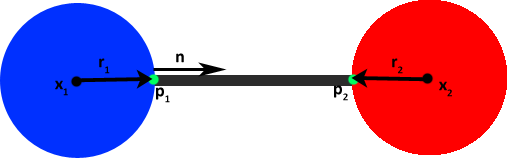
\includegraphics[width=1\textwidth]{pictures/generalConstraint.png}
}
\caption{\label{Fig_constraint}Constraint between two objects}
\end{center}
\end{figure}

~\newline

%Data Definition 1 -DD1 - Mass Normal
\noindent
\begin{minipage}{\textwidth}
\renewcommand*{\arraystretch}{1.5}
\begin{tabular}{| p{\colAwidth} | p{\colBwidth}|}
\hline
\rowcolor[gray]{0.9}
Number& DD\refstepcounter{datadefnum}\thedatadefnum \label{DD_MN}\\
\hline
Label& \bf Mass Normal\\
\hline
Symbol &\ $m_\text{n}$\\
\hline
SI Units &\\
\hline
Equation& $ m_\text{n} = \frac{1}{\frac{1}{m_\text{1}} +
\frac{1}{I_\text{1}}(\textbf r_\text{1} \times \textbf n)^{2}
+ \frac{1}{m_\text{2}} + \frac{1}{I_\text{2}}(\textbf r_\text{2} \times \textbf
n)^{2}}$ \\
\hline
Description & 
$ m_\text{n} $ = Mass normal\\
&$ I_\text{i} $=The moment of inertia of the ith object \\
&$ m_\text{i} $=The mass of the ith object \\
&$\bf n$ = The normal vector between the two constraints (DD\ref{DD_MN}) \\
&$\bf r_\text{i}$ = The vector between the ith object's constraint and its
position (DD\ref{DD_CD})\\
\hline
Sources& \\
\hline
Ref.\ By & IM\ref{IM_C_PinJ}, IM\ref{IM_C_DampedS} \\
\hline
\end{tabular}
\end{minipage}\\

~\newline

%Data Definition 1 -DD1 - Velocity of a point on a rigid body
\noindent
\begin{minipage}{\textwidth}
\renewcommand*{\arraystretch}{1.5}
\begin{tabular}{| p{\colAwidth} | p{\colBwidth}|}
\hline
\rowcolor[gray]{0.9}
Number& DD\refstepcounter{datadefnum}\thedatadefnum \label{DD_VP}\\
\hline
Label& \bf  Velocity of a point on a rigid body\\
\hline
Symbol & $\textbf v_\text{p}$ \\
\hline
SI Units &\\
\hline
Equation& $  \bf v_\text{p} = \omega r_\text{$\perp$} + v $ \\
\hline
Description & 
$ \bf v_\text{p}$ = The velocity of a point on the rigid body\\
&$ \omega $=The angular velocity of the object \\
&$  \bf v $=The velocity of the object \\
&$\bf r$ = The vector between the position of the point and the position of the
object\\
&$\bf r_\text{$\perp$}$ = The vector r rotated counterclockwise by $90^{\circ}$
(DD\ref{DD_PV})\\
\hline
Sources& \\
\hline
Ref.\ By & DD\ref{DD_RV}\\
\hline
\end{tabular}
\end{minipage}\\
~\newline

%Data Definition 1 -DD1 -Relative Velocity
\noindent
\begin{minipage}{\textwidth}
\renewcommand*{\arraystretch}{1.5}
\begin{tabular}{| p{\colAwidth} | p{\colBwidth}|}
\hline
\rowcolor[gray]{0.9}
Number& DD\refstepcounter{datadefnum}\thedatadefnum \label{DD_RV}\\
\hline
Label& \bf Relative Velocity\\
\hline
Symbol & $\textbf r_\text{v}$ \\
\hline
SI Units &\\
\hline
Equation& $ \textbf r_\text{v} = \textbf v_\text{p2} - \textbf v_\text{p1}$
~\newline
Using DD\ref{DD_VP} : $\textbf r_\text{v} = \omega_\text{2}\textbf
r_\text{2$\perp$} + \textbf v_\text{2} - \omega_\text{1}\textbf
r_\text{1$\perp$} - \textbf v_\text{1}$ \\
\hline
Description & 
$ \bf r_\text{v} $ = The relative velocity between the two objects\\
&$ \bf v_\text{pi} $ = The velocity of the point of constraint of the ith
object\\
&$ \omega_\text{i} $=The angular velocity of the ith object \\
&$  \bf v_\text{i} $=The velocity of the ith object \\
&$\bf r_\text{i}$ = The vector between the ith object's constraint and its
center of mass (DD\ref{DD_CD})\\
&$\bf r_\text{i$\perp$}$ = The vector $\textbf r_\text{i}$ rotated
counterclockwise by $90^{\circ}$ (DD\ref{DD_PV})\\
\hline
Sources& \\
\hline
Ref.\ By & IM\ref{IM_C_PinJ}, IM\ref{IM_C_PivotJ}, IM\ref{IM_C_DampedS} \\
\hline
\end{tabular}
\end{minipage}\\
~\newline 

%Data Definition 1 -DD1 -Mass  Matrix
\noindent
\begin{minipage}{\textwidth}
\renewcommand*{\arraystretch}{1.5}
\begin{tabular}{| p{\colAwidth} | p{\colBwidth}|}
\hline
\rowcolor[gray]{0.9}
Number& DD\refstepcounter{datadefnum}\thedatadefnum \label{DD_MT}\\
\hline
Label& \bf Mass Matrix\\
\hline
Symbol &\bf k \\
\hline
SI Units &\\
\hline
Equation& \textbf k =$\begin{bmatrix}
\frac{1}{m_\text{1}} + \frac{1}{m_\text{2}} + \frac{r_\text{1y}^{2}}{I_\text{1}}
+ \frac{r_\text{2y}^{2}}{I_\text{2}} &
\frac{-r_\text{1x} * r_\text{1y}}{I_\text{1}} + \frac{-r_\text{2x} *
r_\text{2y}}{I_\text{2}}\\
\frac{-r_\text{1x} * r_\text{1y}}{I_\text{1}} + \frac{-r_\text{2x} *
r_\text{2y}}{I_\text{2}} &
\frac{1}{m_\text{1}} + \frac{1}{m_\text{2}} + \frac{r_\text{1x}^{2}}{I_\text{1}}
+ \frac{r_\text{2x}^{2}}{I_\text{2}}\\
        \end{bmatrix}$ \\
\hline
Description & 
\textbf k = Mass Matrix\\
&$\bf r_\text{i}$ = The vector between the ith object's constraint and its
position (DD\ref{DD_CD})\\
& $I_\text{i}$ =The moment of inertia of the ith object \\
& $m_\text{i}$ =The mass of the ith object \\
& $r_\text{ix} $= The x component of the vector $\textbf r_\text{i}$ \\
& $r_\text{iy} $= The y component of the vector $\textbf r_\text{i}$ \\

\hline
Sources& \\
\hline
Ref.\ By & IM\ref{IM_C_PivotJ}\\
\hline
\end{tabular}
\end{minipage}\\

%Data Definition 1 -DD1 - Error Correction
\noindent
\begin{minipage}{\textwidth}
\renewcommand*{\arraystretch}{1.5}
\begin{tabular}{| p{\colAwidth} | p{\colBwidth}|}
\hline
\rowcolor[gray]{0.9}
Number& DD\refstepcounter{datadefnum}\thedatadefnum \label{DD_EC}\\
\hline
Label& \bf Error Correction\\
\hline
Symbol & b \\
\hline
SI Units &\\
\hline
Equation& $  \textbf b = \frac{k_\text{erp}}{\Delta t}e_\text{c}$ \\
\hline
Description & 
The error correction term is used to fix any errors in the position/orientation
of the object.
An impulse is applied to the velocities and angular velocities of the object.
The new position and
orientation are then calculated. Due to numerical errors the position and
orientation of the
object can differ from the true location. \\

&$ \textbf b $ = The error correction\\
&$ k_\text{erp} $= The error reduction parameter. This value is 0 $\le
k_\text{erp} \le 1.$ A $ k_\text{erp}$ of 1 means to fix the error immediately,
while a value of 0 means to
not fix the error at all.  \\
&$ \Delta t $ = The change in time between frames \\
&$ e_\text{c}$ = The calculation of the error. Each constraint calculates this
value differently.\\
\hline
Sources& \\
\hline
Ref.\ By & IM\ref{IM_C_PinJ}, IM\ref{IM_C_SlideJ}, IM\ref{IM_C_PivotJ},
IM\ref{IM_C_RotaryJ}, IM\ref{IM_C_RatchetJ}, IM\ref{IM_C_GearJ}\\
\hline
\end{tabular}
\end{minipage}\\

~\newline

%Data Definition 1 -DD1 - Perpendicular Vector
\noindent
\begin{minipage}{\textwidth}
\renewcommand*{\arraystretch}{1.5}
\begin{tabular}{| p{\colAwidth} | p{\colBwidth}|}
\hline
\rowcolor[gray]{0.9}
Number& DD\refstepcounter{datadefnum}\thedatadefnum \label{DD_PV}\\
\hline
Label& \bf Perpindicular Vector\\
\hline
Symbol & $\textbf v_\text{$\perp$}$ \\
\hline
SI Units &\\
\hline
Equation& $ \textbf v_\text{$\perp$} = \begin{bmatrix}
       -v_\text{y} \\
       v_\text{x}\\
        \end{bmatrix} $ \\
\hline
Description & 
The perpendicular vector is the vector \textbf v rotated counterclockwise by
$90^{ \degree}$ \\

\hline
Sources& \\
\hline
Ref.\ By & IM\ref{IM_C_PinJ},  IM\ref{IM_C_PivotJ}, IM\ref{IM_C_DampedS} \\
\hline
\end{tabular}
\end{minipage}\\

%Data Definition 1 -DD1 - 2D Cross Product
\noindent
\begin{minipage}{\textwidth}
\renewcommand*{\arraystretch}{1.5}
\begin{tabular}{| p{\colAwidth} | p{\colBwidth}|}
\hline
\rowcolor[gray]{0.9}
Number& DD\refstepcounter{datadefnum}\thedatadefnum \label{DD_CP}\\
\hline
Label& \bf2D Cross Product\\
\hline
Symbol & $\textbf u \times \textbf v$ \\
\hline
SI Units &\\
\hline
Equation& $ \textbf u \times \textbf v = u_\text{x}v_\text{y} -
u_\text{y}v_\text{x}$ \\
\hline
Description & 
For the purpose of this document, the cross product of two 2D vectors 
will result in a scalar quantity.  \\

&$ \textbf u$ = A 2D vector\\
&$ \textbf v$ = A 2D vector\\
&$ u_\text{x}, u_\text{y}$ = The x and y components of the vector \textbf u \\
&$ v_\text{x}, v_\text{y}$ = The x and y components of the vector \textbf v \\
\hline
Sources& \\
\hline
Ref.\ By & IM\ref{IM_C_PinJ},  IM\ref{IM_C_PivotJ}, IM\ref{IM_C_DampedS} \\
\hline
\end{tabular}
\end{minipage}\\


\subsection{Instance Models}
%Instance Model  1 -IM1- Constraint
\noindent
\begin{minipage}{\textwidth}
\renewcommand*{\arraystretch}{1.5}
\begin{tabular}{| p{\colAwidth} | p{\colBwidth}|}
  \hline
  \rowcolor[gray]{0.9}
  Number& IM\refstepcounter{instnum}\theinstnum \label{IM_CONSTRAINT}\\
  \hline
  Label& \bf Constraint on a 2D rigid body \\
  \hline
Input&$\bf {J}, p_\text{1},p_\text{2}, x_\text{1},x_\text{2}, v_\text{1},
v_\text{2}, \textnormal I_\text{1},\textnormal I_\text{2}, \textnormal
m_\text{1}, \textnormal m_\text{2},
   \omega_\text{1},  \omega_\text{2}  $\\
  \hline
Output &$ \bf v'_\text{1}, v'_\text{2}, \boldsymbol \omega'_\text{1},
\boldsymbol \omega'_\text{2} $
  such that: \\
 
  & $\bf v'_\text{1} =  v_\text{1} + \frac{-J}{ \textnormal m_\text{1}}$\\
  & $\bf v'_\text{2} =  v_\text{2} + \frac{J}{ \textnormal m_\text{2}}$\\
  
& $\bf \omega'_\text{1} = \omega_\text{1} + \frac{-r_\text{1} \times
J}{\textnormal I_\text{1}}$\\
& $\bf \omega'_\text{2} = \omega_\text{2} + \frac{r_\text{2} \times
J}{\textnormal I_\text{2}}$\\
  
  \hline
 Description &
$ \textbf J $= The impulse acting on the constraint \\
&$ \textbf p_\text{i} $=The point where the ith object is constrained \\
&$ \textbf x_\text{i} $=The position of the ith object\\
&$ \textbf v_\text{i} $=The old velocity of the ith object \\
&$ \omega_\text{i} $=The old angular velocity of the ith object \\
&$ \textbf r_\text{i} $=The vector between the ith object's constraint and its
position (DD\ref{DD_CD})\\
&$  I_\text{i} $=The moment of inertia of the ith object\\
&$  m_\text{i} $=The mass of the ith object \\
&$ \textbf  v'_\text{i} $=The new velocity of the ith object \\
&$ \omega'_\text{i} $=The new angular velocity of the ith object \\

&The following instance models use the same input and output as described above.The impulse for each constraint is calculated differently and is outlined in
the following instance models. \\
  \hline  
  Sources &\\
  \hline
Ref.\ By & IM\ref{IM_C_PinJ}, IM\ref{IM_C_SlideJ}, IM\ref{IM_C_PivotJ},
IM\ref{IM_C_GrooveJ}, IM\ref{IM_C_DampedS} \\
  \hline
\end{tabular}
\end{minipage}\\
~\newline

\subsubsection {Derivation of the velocity and angular velocity}

The impulse on an object is equal to the change in its linear momentum, that is:\begin{equation*}
\textbf J = \Delta \textbf P 
\end{equation*}

\noindent 
Using GD\ref{GD_M}:
\begin{equation*}
\textbf J  = m\Delta \textbf v = m(\textbf v' - \textbf v)
\end{equation*}

\noindent
Rearrange:
\begin{equation*}
\bf v' =  v + \frac{J}{ \textnormal m}
\end{equation*}

\noindent
The angular momentum of a particle is equal to the cross product of the position 
vector of the particle and the linear momentum. That is:
\begin{equation*}
\Delta L = \textbf r \times \Delta \textbf P = \textbf r  \times \textbf J 
\end{equation*}

\noindent 
Using GD\ref{GD_M}:
\begin{equation*}
 \textbf r  \times  \textbf J  = I \Delta \omega = I(\omega'-\omega)
\end{equation*}

\noindent
Rearrange: 
\begin{equation*}
\omega'=   \omega + \frac{\textbf r \times \textbf J}{\textnormal I}
\end{equation*}

\noindent
Newton's Third Law of motion says that the impulse felt by one object is
equal and opposite the impulse felt by the other object.


\begin{equation*}
\bf v'_\text{1} =  v_\text{1} + \frac{-J}{ \textnormal m_\text{1}}
\end{equation*}

\begin{equation*}
\bf v'_\text{2} =  v_\text{2} + \frac{J}{ \textnormal m_\text{2}}
  \end{equation*}
  
\begin{equation*}
\bf \omega'_\text{1} = \omega_\text{1} + \frac{-r_\text{1} \times J}{\textnormal
I_\text{1}}
  \end{equation*}
  
\begin{equation*}
\bf \omega'_\text{2} = \omega_\text{2} + \frac{r_\text{2} \times J}{\textnormal
I_\text{2}}
  \end{equation*}

\subsubsection{Pin joint} \label{SecConstraintFig}
A pin joint acts as a bar between two objects. The two constraints on 
the objects  are always the same distance apart. 
The objects are able to rotate around the constraint. 
Figure \ref{Fig_pinJoint} shows an example of a pin joint.

~\newline

%Instance Model  2 -IM2- Pin Joint
\noindent
\begin{minipage}{\textwidth}
\renewcommand*{\arraystretch}{1.5}
\begin{tabular}{| p{\colAwidth} | p{\colBwidth}|}
  \hline
  \rowcolor[gray]{0.9}
  Number& IM\refstepcounter{instnum}\theinstnum \label{IM_C_PinJ}\\
  \hline
  Label& \bf Pin Joint\\
  \hline
  Input& IM\ref{IM_CONSTRAINT}\\ 
  \hline
  Output&$ \bf J $ \\
  \hline
  Description &
The impulse for a pin joint is calculated as: \\
&$\textbf J = ((-b - \textbf r_\text{v} \cdot \textbf n) m_\text{n})\textbf n$\\
& b = error correction: $\frac{k_\text{erp}}{\Delta t} (\bf |p_\text{2} -
p_\text{1}| - |(x_\text{2} + r_\text{2}) - (x_\text{1} + r_\text{1})|)$
(DD\ref{DD_EC})\\
& $\textbf r_\text{v} $= relative velocity (DD\ref{DD_RV})\\
& \textbf n = The normal vector between the two constraints  (DD\ref{DD_VN})\\
& $m_\text{n}$ = mass normal (DD\ref{DD_MN})\\

  \hline  
  Sources &\\
  \hline
Ref.\ By & \\
  \hline
\end{tabular}
\end{minipage}\\
~\newline

\begin{figure}[h!]
\begin{center}
%\rotatebox{-90}
{
 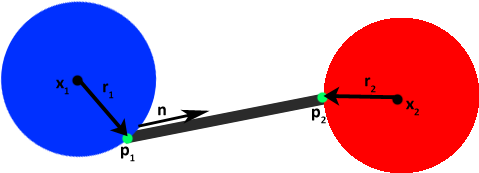
\includegraphics[width=0.75\textwidth]{pictures/pinJoint.png}
}
\caption{\label{Fig_pinJoint}Pin joint between two objects}
\end{center}
\end{figure}

\subsubsection{Derivation of the Impulse on a Pin Joint}
A pin joint acts as a bar between the two objects. The relative velocities 
(DD\ref{DD_RV})
between the two objects in the direction of the constraint 
should equal zero. That is:

\begin{equation}
(\textbf v'_\text{2} + \omega'_\text{2}\textbf r_\text{2$\perp$} - \textbf
v'_\text{1} - \omega'_\text{1}\textbf r_\text{1$\perp$}) \cdot \textbf n = 0
\label{eq:rv}
\end{equation}

\noindent
The updated velocities and angular velocities should equal:

\begin{equation*}
\bf v'_\text{1} =  v_\text{1} + \frac{-J}{ \textnormal m_\text{1}}
\end{equation*}

\begin{equation*}
\bf v'_\text{2} =  v_\text{2} + \frac{J}{ \textnormal m_\text{2}}
  \end{equation*}
  
\begin{equation*}
\bf \omega'_\text{1} = \omega_\text{1} + \frac{-r_\text{1} \times J}{\textnormal
I_\text{1}}
  \end{equation*}
  
\begin{equation*}
\bf \omega'_\text{2} = \omega_\text{2} + \frac{r_\text{2} \times J}{\textnormal
I_\text{2}}
  \end{equation*}


\noindent
The impulse should only be applied in the direction of the constraint: 
\begin{equation}
\textbf J = J\textbf n \label{eq:imp}
\end{equation}

\noindent
Substituting the above equations into Eq\ref{eq:rv}:

\begin{equation*}
(\textbf v_\text{2} + \frac{J\textbf n}{ \textnormal m_\text{2}} + 
( \omega_\text{2} + \frac{\textbf r_\text{2} \times  J\textbf n}{
I_\text{2}})\textbf r_\text{2$\perp$} -
\textbf v_\text{1} + \frac{  J\textbf n}{ \textnormal m_\text{1}} +  
( - \omega_\text{1} + \frac{\textbf r_\text{1} \times 
J\textbf n}{I_\text{1}})\textbf r_\text{1$\perp$}) \cdot \textbf n = 0
\end{equation*}

\noindent
Factor out the impulse 

\begin{equation*}
J\textbf n \cdot \textbf n (\frac{\textbf n}{ \textnormal m_\text{2}} + \frac{(\textbf r_\text{2} \times
\textbf n) \textbf r_\text{2$\perp$} }{I_\text{2}} + \frac{\textbf n}{
\textnormal m_\text{1}} + \frac{(\textbf r_\text{1} \times \textbf n) \textbf
r_\text{1$\perp$} }{I_\text{1}} ) \cdot \textbf n +
\textbf v_\text{2}\cdot \textbf n + \omega_\text{2}\textbf r_\text{2$\perp$}
\cdot \textbf n -
\textbf v_\text{1} \cdot \textbf n - \omega_\text{1}\textbf r_\text{1$\perp$}
\cdot \textbf n= 0
\end{equation*}

\noindent
Using DD\ref{DD_PV} and DD\ref{DD_CP}
\begin{equation*}
\textbf r_\text{i$\perp$} \cdot \textbf n = \textbf r_\text{i} \times \textbf n
\end{equation*}

\noindent
Simplifying
\begin{equation*}
J (\frac{1}{ \textnormal m_\text{2}} + \frac{(\textbf r_\text{2} \times \textbf
n)^{2} }{I_\text{2}} + \frac{1}{ \textnormal m_\text{1}} + \frac{(\textbf
r_\text{1} \times \textbf n) ^{2}}{I_\text{1}} )+
\textbf v_\text{2}\cdot \textbf n + \omega_\text{2}\textbf r_\text{2$\perp$}
\cdot \textbf n -
\textbf v_\text{1} \cdot \textbf n - \omega_\text{1}\textbf r_\text{1$\perp$}
\cdot \textbf n= 0
\end{equation*}

\noindent
Rearrange: 

\begin{equation*}
J =\frac{( \textbf v_\text{1} + \omega_\text{1}\textbf r_\text{1$\perp$} -
\textbf v_\text{2}
 - \omega_\text{2}\textbf r_\text{2$\perp$} ) \cdot \textbf n}
{\frac{1}{ \textnormal m_\text{2}} + \frac{(\textbf r_\text{2} \times\textbf n)
^{2}}{I_\text{2}} + \frac{1}{ \textnormal m_\text{1}} + \frac{(\textbf
r_\text{1} \times \textbf n) ^{2}}{I_\text{1}}}
\end{equation*}

\noindent
Using DD\ref{DD_RV} and DD\ref{DD_MN} the above equation simplifies to: 
\begin{equation*}
J = (-\textbf r_\text{v}\cdot \textbf n)m_\text{n}
\end{equation*}

\noindent
Substituting the above equation into Eq\ref{eq:imp}:
\begin{equation*}
\textbf J = ((-\textbf r_\text{v}\cdot \textbf n)m_\text{n})\textbf n
\end{equation*}


\noindent
As mentioned in DD\ref{DD_EC} an error correction term must be added to the
velocity to fix potential issues with the position:
\begin{equation*}
\textbf J = ((-b -\textbf r_\text{v}\cdot \textbf n)m_\text{n})\textbf n
\end{equation*}

\subsubsection{Slide joint} \label{SecConstraintFig}
A slide joint is similar to a pin joint but has a minimum and maximum distance.
Figure \ref{Fig_slideJoint} shows an example of a slide joint
~\newline

%Instance Model  3 -IM3-  Slide Joint
\noindent
\begin{minipage}{\textwidth}
\renewcommand*{\arraystretch}{1.5}
\begin{tabular}{| p{\colAwidth} | p{\colBwidth}|}
  \hline
  \rowcolor[gray]{0.9}
  Number& IM\refstepcounter{instnum}\theinstnum \label{IM_C_SlideJ}\\
  \hline
  Label& \bf Slide Joint\\
  \hline
  Input& IM\ref{IM_CONSTRAINT},  max, min\\ 
  \hline
  Output&$ \bf J $ \\
  \hline
  Description 
&  Impulse is calculated the same as IM\ref{IM_C_PinJ}. Except\\
  
& b = $ \begin{cases}
\frac{k_\text{erp}}{\Delta t} (|\textbf p_\text{2} - \textbf p_\text{1}| - max)
& \text { if }|\textbf p_\text{2}-\textbf p_\text{1}| > max\\
\frac{k_\text{erp}}{\Delta t} (min - |\textbf p_\text{2} - \textbf p_\text{1}| )
& \text { if }|\textbf p_\text{2}-\textbf p_\text{1}| < min \\
  \text{no impulse} & \text{otherwise}\\
  \end{cases}$ \\
  
& b = Error correction:   (DD\ref{DD_EC})\\
& min =  The minimum distance the two objects can be from each other \\
& max =  The maximum distance the two objects can be from each other \\

  \hline  
  Sources &\\
  \hline
Ref.\ By & \\
  \hline
\end{tabular}
\end{minipage}\\
~\newline

\begin{figure}[htbp]
\begin{center}
%\rotatebox{-90}
{
 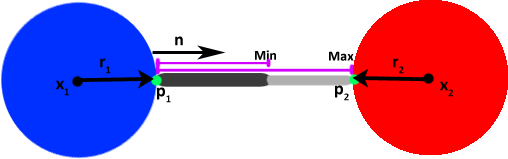
\includegraphics[width=0.75\textwidth]{pictures/slideJoint.png}
}
\caption{\label{Fig_slideJoint} Slide joint between two objects}
\end{center}
\end{figure}


\subsubsection{Pivot joint} \label{SecConstraintFig}
A pivot joint holds two constraint  points together.
The rotational point is not fixed.
Figure \ref{Fig_pivotJoint} shows an example of a pivot joint
~\newline

%Instance Model  4 -IM4- Pivot joint
\noindent
\begin{minipage}{\textwidth}
\renewcommand*{\arraystretch}{1.5}
\begin{tabular}{| p{\colAwidth} | p{\colBwidth}|}
  \hline
  \rowcolor[gray]{0.9}
  Number& IM\refstepcounter{instnum}\theinstnum \label{IM_C_PivotJ}\\
  \hline
  Label& \bf Pivot Joint\\
  \hline
  Input& IM\ref{IM_CONSTRAINT}\\ 
  \hline
  Output&$ \bf J $ \\
  \hline
  Description   &
The impulse for a pivot joint is calculated as: \\
  &$\textbf J = (-\textbf b -\textbf  r_\text{v})\textbf k^{-1}$ \\

&\textbf b = Error correction: $\frac{k_\text{erp}}{\Delta t} (\textbf
p_\text{2} - \textbf p_\text{1}) $ (DD\ref{DD_EC})\\
& $\textbf r_\text{v} $= Relative velocity (DD\ref{DD_RV})\\
&\textbf  k = Mass matrix(DD\ref{DD_MT})\\
  \hline  
  Sources &\\
  \hline
Ref.\ By & \\
  \hline
\end{tabular}
\end{minipage}\\

\begin{figure}[htbp]
\begin{center}
%\rotatebox{-90}
{
 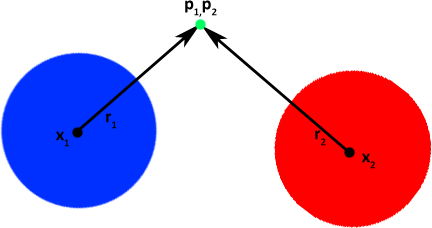
\includegraphics[width=0.75\textwidth]{pictures/pivotJoint.png}
}
\caption{\label{Fig_pivotJoint}Pivot joint between two objects}
\end{center}
\end{figure}

\subsubsection{Derivation of the Impulse on a Pivot Joint}
The relative velocities  (DD\ref{DD_RV})
between the two objects should equal zero. That is

\begin{equation}
(\textbf v'_\text{2} + \omega'_\text{2}\textbf r_\text{2$\perp$} - \textbf
v'_\text{1} - \omega'_\text{1}\textbf r_\text{1$\perp$}) = 0 \label{eq:pivotrv}
\end{equation}


\noindent
The updated velocities and angular velocities should equal:

\begin{equation*}
\bf v'_\text{1} =  v_\text{1} + \frac{-J}{ \textnormal m_\text{1}}
\end{equation*}

\begin{equation*}
\bf v'_\text{2} =  v_\text{2} + \frac{J}{ \textnormal m_\text{2}}
  \end{equation*}
  
\begin{equation*}
\omega'_\text{1} = \omega_\text{1} + \frac{-\textbf r_\text{1} \times \textbf
J}{I_\text{1}}
  \end{equation*}
  
\begin{equation*}
\omega'_\text{2} = \omega_\text{2} + \frac{\textbf r_\text{2} \times \textbf
J}{I_\text{2}}
  \end{equation*}

\noindent
Substituting the above equations into Eq\ref{eq:pivotrv}:

\begin{equation*}
\textbf v_\text{2} + \frac{\textbf J}{ \textnormal m_\text{2}} + 
( \omega_\text{2} + \frac{\textbf r_\text{2} \times \textbf
J}{I_\text{2}})\textbf r_\text{2$\perp$} -
\textbf v_\text{1} + \frac{\textbf J}{ \textnormal m_\text{1}} +  
( - \omega_\text{1} + \frac{\textbf r_\text{1} \times \textbf
J}{I_\text{1}})\textbf r_\text{1$\perp$}= 0
\end{equation*}

\noindent
Rearrange

\begin{equation*}
\textbf J(\frac{1}{ \textnormal m_\text{2}} + \frac{1}{ \textnormal
m_\text{1}})+ \frac{(\textbf r_\text{2} \times \textbf J)}{I_\text{2}}\textbf
r_\text{2$\perp$} + \frac{(\textbf r_\text{1} \times \textbf J) }{I_\text{1}}
\textbf r_\text{1$\perp$}
= \textbf v_\text{1} + \omega_\text{1} \textbf r_\text{1$\perp$} - \textbf
v_\text{2} - \omega_\text{2}\textbf r_\text{2$\perp$}
\end{equation*}

\noindent
Expand cross product and perpendicular vector using DD\ref{DD_CP} and
DD\ref{DD_PV}

\begin{equation*}
\textbf J(\frac{1}{ \textnormal m_\text{2}} + \frac{1}{ \textnormal
m_\text{1}})+ \frac{(r_\text{2x}J_\text{y} - r_\text{2y}J_\text{x})}{I_\text{2}}
 \begin{bmatrix}
         -r_\text{2y} \\
        r_\text{2x} \\
\end{bmatrix} + \frac{(r_\text{1x}J_\text{y} -
r_\text{1y}J_\text{x})}{I_\text{1}}
 \begin{bmatrix}
         -r_\text{1y} \\
        r_\text{1x} \\
        \end{bmatrix} 
= \textbf v_\text{1} + \omega_\text{1} \textbf r_\text{1$\perp$} - \textbf
v_\text{2} - \omega_\text{2}\textbf r_\text{2$\perp$}
\end{equation*}

\noindent
Multiply the cross product by the perpendicular vector
\begin{equation*}
\textbf J(\frac{1}{ \textnormal m_\text{2}} + \frac{1}{ \textnormal
m_\text{1}})+ \frac{
 \begin{bmatrix}
         J_\text{x}r_\text{2y}^{2} -J_\text{y}r_\text{2x}r_\text{2y}\\
        J_\text{y}r_\text{2x}^{2} -J_\text{x}r_\text{2x}r_\text{2y} \\
        \end{bmatrix}}{I_\text{2}} + \frac{
 \begin{bmatrix}
         J_\text{x}r_\text{1y}^{2} -J_\text{y}r_\text{1x}r_\text{1y}\\
        J_\text{y}r_\text{1x}^{2} -J_\text{x}r_\text{1x}r_\text{1y} \\
        \end{bmatrix}}{I_\text{1}} 
= \textbf v_\text{1} + \omega_\text{1} \textbf r_\text{1$\perp$} - \textbf
v_\text{2} - \omega_\text{2}\textbf r_\text{2$\perp$}
\end{equation*}

\noindent
Factor out the impulse
\begin{equation*}
\textbf J\begin{bmatrix}
\frac{1}{ \textnormal m_\text{2}} + \frac{1}{ \textnormal m_\text{1}} & 0\\0 
& \frac{1}{ \textnormal m_\text{2}} + \frac{1}{ \textnormal m_\text{1}}\\       
 \end{bmatrix} + \textbf J
 \begin{bmatrix}
\frac{ r_\text{2y}^{2}}{I_\text{2}} &
\frac{-r_\text{2x}r_\text{2y}}{I_\text{2}}\\
\frac{-r_\text{2x}r_\text{2y}}{I_\text{2}} &
\frac{r_\text{2x}^{2}}{I_\text{2}}\\
        \end{bmatrix} + \textbf J
 \begin{bmatrix}
\frac{ r_\text{1y}^{2}}{I_\text{1}} &
\frac{-r_\text{1x}r_\text{1y}}{I_\text{1}}\\
\frac{-r_\text{1x}r_\text{1y}}{I_\text{1}} &
\frac{r_\text{1x}^{2}}{I_\text{1}}\\
        \end{bmatrix} 
= \textbf v_\text{1} + \omega_\text{1} \textbf r_\text{1$\perp$} - \textbf
v_\text{2} - \omega_\text{2}\textbf r_\text{2$\perp$}
\end{equation*}

\noindent
Add the matrices together:

\begin{equation*}
\textbf J
\begin{bmatrix}
\frac{1}{ \textnormal m_\text{2}} + \frac{1}{ \textnormal m_\text{1}}+
\frac{r_\text{1y}^{2}}{I_\text{1}} + \frac{r_\text{2y}^{2}}{I_\text{2}} &
\frac{-r_\text{1x} * r_\text{1y}}{I_\text{1}} + \frac{-r_\text{2x} *
r_\text{2y}}{I_\text{2}}\\
\frac{-r_\text{1x} * r_\text{1y}}{I_\text{1}} + \frac{-r_\text{2x} *
r_\text{2y}}{I_\text{2}} &
\frac{1}{ \textnormal m_\text{2}} + \frac{1}{ \textnormal m_\text{1}}+
\frac{r_\text{1x}^{2}}{I_\text{1}} + \frac{r_\text{2x}^{2}}{I_\text{2}}\\
        \end{bmatrix}
= \textbf v_\text{1} + \omega_\text{1} \textbf r_\text{1$\perp$} - \textbf
v_\text{2} - \omega_\text{2}\textbf r_\text{2$\perp$}
\end{equation*}

\noindent
Rearrange:
\begin{equation*}
\textbf J 
= (\textbf v_\text{1} + \omega_\text{1} \textbf r_\text{1$\perp$} - \textbf
v_\text{2} - \omega_\text{2}\textbf r_\text{2$\perp$})
\begin{bmatrix}
\frac{1}{ \textnormal m_\text{2}} + \frac{1}{ \textnormal m_\text{1}}+
\frac{r_\text{1y}^{2}}{I_\text{1}} + \frac{r_\text{2y}^{2}}{I_\text{2}} &
\frac{-r_\text{1x} * r_\text{1y}}{I_\text{1}} + \frac{-r_\text{2x} *
r_\text{2y}}{I_\text{2}}\\
\frac{-r_\text{1x} * r_\text{1y}}{I_\text{1}} + \frac{-r_\text{2x} *
r_\text{2y}}{I_\text{2}} &
\frac{1}{ \textnormal m_\text{2}} + \frac{1}{ \textnormal m_\text{1}}+
\frac{r_\text{1x}^{2}}{I_\text{1}} + \frac{r_\text{2x}^{2}}{I_\text{2}}\\
        \end{bmatrix}^{-1}
\end{equation*}

\noindent
Simplifying using DD\ref{DD_MT} and DD\ref{DD_RV}:
\begin{equation*}
\textbf J = (-\textbf r_\text{v}) \textbf k^{-1}
\end{equation*}


\noindent
As mentioned in DD\ref{DD_EC} an error correction term must be added to the
velocity to fix potential issues with the position:
\begin{equation*}
\textbf J =(-\textbf b -\textbf r_\text{v}) \textbf k^{-1}
\end{equation*}

\subsubsection{Groove joint} \label{SecConstraintFig}
A groove joint is similar to a pivot joint, except one of the constraints
 is a line segment that the pivot can slide in.
Figure \ref{Fig_grooveJoint} shows an example of a groove joint.
~\newline

%Instance Model  5  -IM5-  Groove Joint
\noindent
\begin{minipage}{\textwidth}
\renewcommand*{\arraystretch}{1.5}
\begin{tabular}{| p{\colAwidth} | p{\colBwidth}|}
  \hline
  \rowcolor[gray]{0.9}
  Number& IM\refstepcounter{instnum}\theinstnum \label{IM_C_GrooveJ}\\
  \hline
  Label& \bf Groove Joint\\
  \hline
  Input& IM$\ref{IM_CONSTRAINT}, \bf g_\text{a}, g_\text{b}$\\ 
  \hline
  Output&$ \bf J $ \\
  \hline
  Description 
 &Impulse is calculated the same as \ref{IM_C_PivotJ} except:\\

& $\bf r_\text{1} =  \begin{cases}
\textbf g_\text{a} - \textbf x_\text{1} & \text { if } \textbf p_\text{2} \times
\textbf n\le \textbf g_\text{a} \times \textbf n \\
\textbf g_\text{b} - \textbf x_\text{1} & \text { if } \textbf p_\text{2} \times
\textbf n \ge \textbf g_\text{b} \times \textbf n \\
- (\textbf p_\text{2} \times \textbf n) \textbf n_\text{$\perp$} + \textbf
n(\textbf g_\text{a}\cdot \textbf n) - \textbf x_\text{1} & \text{otherwise}\\
  \end{cases} $\\

&$\textbf g_\text{a}$ = The point the line segment begins \\ 
&$\textbf g_\text{b}$ = The point the line segment ends \\
&$\textbf n$ = The normalized vector perpendicular to the line segment\\

  \hline  
  Sources &\\
  \hline
Ref.\ By & \\
  \hline
\end{tabular}
\end{minipage}\\
~\newline

\begin{figure}[htbp]
\begin{center}
%\rotatebox{-90}
{
 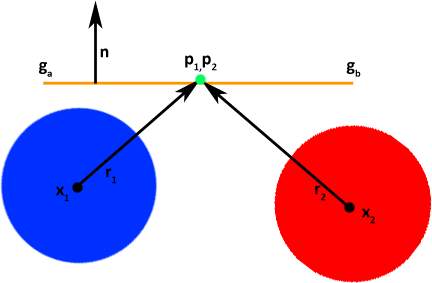
\includegraphics[width=0.75\textwidth]{pictures/grooveJoint.png}
}
\caption{\label{Fig_grooveJoint}Groove joint between two objects}
\end{center}
\end{figure}

\subsubsection{Damped Spring} \label{SecConstraintFig}
A spring between two objects. The spring tries to stay at its
rest length (d). 
Figure \ref{Fig_dampedSpring} shows an example of a damped spring.
~\newline

%Instance Model  6 -IM6- Damped Spring
\noindent
\begin{minipage}{\textwidth}
\renewcommand*{\arraystretch}{1.5}
\begin{tabular}{| p{\colAwidth} | p{\colBwidth}|}
  \hline
  \rowcolor[gray]{0.9}
  Number& IM\refstepcounter{instnum}\theinstnum \label{IM_C_DampedS}\\
  \hline
  Label& \bf Damped Spring\\
  \hline
  Input& IM\ref{IM_CONSTRAINT},$\zeta$, k , d\\ 
  \hline
  Output&$ \bf J $ \\
  \hline
  Description 
& \textbf J= $( k(|\textbf p_\text{2} - \textbf p_\text{1}| - d)\Delta
t$)\textbf n - (($\textbf r_\text{v} \cdot \textbf n (1 - e^{-\zeta
\frac{1}{m_\text{n}}t}) m_\text{n})\textbf n)$ \\

&$ k $= Spring stiffness\\
&$ \textbf p_\text{i} $= Position of the constraint of the ith object\\
&$ d$= Rest length of the spring\\
&$ \textbf r_\text{v} $= Relative velocity (DD\ref{DD_RV})\\
& \textbf n =The normal vector between the two constraints (DD\ref{DD_VN})\\
& $m_\text{n}$ = Mass normal (DD\ref{DD_MN})\\
& t = Time\\
&$ \Delta t $= Time in between frames\\
&$ \zeta$ =Damping coefficient\\
  \hline  
  Sources &\\
  \hline
Ref.\ By & \\
  \hline
\end{tabular}
\end{minipage}\\
~\newline

\begin{figure}[htbp]
\begin{center}
%\rotatebox{-90}
{
 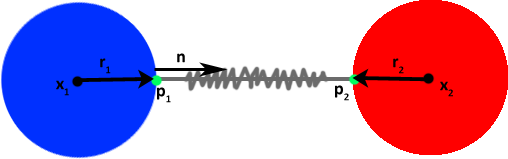
\includegraphics[width=0.75\textwidth]{pictures/DampedSpring.png}
}
\caption{\label{Fig_dampedSpring}Damped spring between two objects}
\end{center}
\end{figure}

\subsubsection{Derivation of the Impulse on a Damped Spring}
Acts as a spring between the two objects. Hooke's law states:
\begin{equation*}
\textbf F = k\textbf X
\end{equation*}

\noindent
Where x is the amount the spring is displaced from its rest length. 
\begin{equation*}
\textbf F = k(|\textbf p_\text{2} - \textbf p_\text{1}| - d)\textbf n
\end{equation*}

\noindent
Impulse is a force acting over an interval of time: 
\begin{equation}
\textbf J = k\Delta t(|\textbf p_\text{2} - \textbf p_\text{1}| - d)\textbf n
\label{eq:hooke}
\end{equation}

\noindent
With no damping ($\zeta=0$), the above equation would be the impulse. 
With damping, an impulse to calculate the damping is needed.
The updated relative velocities 
between the two objects in the direction of the constraint should 
equal the old relative velocities multiplied by a damping value ($\gamma$).
That is:

\begin{equation}
(\textbf v'_\text{2} + \omega'_\text{2}\textbf r_\text{2$\perp$} - \textbf
v'_\text{1} - \omega'_\text{1}\textbf r_\text{1$\perp$}) \cdot \textbf n =
\gamma(\textbf v_\text{2} + \omega_\text{2}\textbf r_\text{2$\perp$} - \textbf
v_\text{1} - \omega_\text{1}\textbf r_\text{1$\perp$}) \cdot \textbf n
\label{eq:rv_s}
\end{equation}

\noindent
The updated velocities and angular velocities should equal:

\begin{equation*}
\bf v'_\text{1} =  v_\text{1} + \frac{-J}{ \textnormal m_\text{1}}
\end{equation*}

\begin{equation*}
\bf v'_\text{2} =  v_\text{2} + \frac{J}{ \textnormal m_\text{2}}
  \end{equation*}
  

\begin{equation*}
\omega'_\text{1} = \omega_\text{1} + \frac{-\textbf r_\text{1} \times \textbf
J}{I_\text{1}}
  \end{equation*}
  
\begin{equation*}
\omega'_\text{2} = \omega_\text{2} + \frac{\textbf r_\text{2} \times \textbf
J}{I_\text{2}}
  \end{equation*}


\noindent
The impulse should only be applied in the direction of the constraint: 
\begin{equation}
\textbf J = J\textbf n \label{eq:imp2}
\end{equation}

\noindent
Substituting the above equations into Eq\ref{eq:rv_s}:

\begin{equation*}
(\textbf v_\text{2} + \frac{ J\textbf n}{ \textnormal m_\text{2}} + 
( \omega_\text{2} + \frac{ \textbf r_\text{2} \times J\textbf n}{I_\text{2}})\textbf r_\text{2$\perp$} -
\textbf v_\text{1} + \frac{J\textbf n}{ \textnormal m_\text{1}} +  
( - \omega_\text{1} + \frac{ \textbf r_\text{1} \times J\textbf n}{I_\text{1}})\textbf r_\text{1$\perp$}) \cdot \textbf n =\gamma(\textbf
v_\text{2} + \omega_\text{2}\textbf r_\text{2$\perp$} - \textbf v_\text{1} -
\omega_\text{1}\textbf r_\text{1$\perp$}) \cdot \textbf n
\end{equation*}

\noindent
Factor out the impulse 

\begin{equation*}
J\textbf n \cdot \textbf n(\frac{\textbf n}{ \textnormal m_\text{2}} + \frac{(\textbf r_\text{2} \times
\textbf n) \textbf r_\text{2$\perp$} }{I_\text{2}} + \frac{\textbf n}{
\textnormal m_\text{1}} + \frac{(\textbf r_\text{1} \times \textbf n) \textbf
r_\text{1$\perp$} }{I_\text{1}} ) \cdot \textbf n +
\textbf v_\text{2}\cdot \textbf n + \omega_\text{2}\textbf r_\text{2$\perp$}
\cdot \textbf n -
\textbf v_\text{1} \cdot \textbf n - \omega_\text{1}\textbf r_\text{1$\perp$}
\cdot \textbf n= \gamma(\textbf v_\text{2} + \omega_\text{2}\textbf
r_\text{2$\perp$} - \textbf v_\text{1} - \omega_\text{1}\textbf
r_\text{1$\perp$}) \cdot \textbf n
\end{equation*}

\noindent
Using DD\ref{DD_PV} and DD\ref{DD_CP}
\begin{equation*}
\textbf r_\text{i$\perp$} \cdot \textbf n = \textbf r_\text{i} \times \textbf n
\end{equation*}

\noindent
Simplifying

\begin{equation*}
J(\frac{1}{ \textnormal m_\text{2}} + \frac{(\textbf r_\text{2} \times \textbf
n)^{2} }{I_\text{2}} + \frac{1}{ \textnormal m_\text{1}} + \frac{(\textbf
r_\text{1} \times \textbf n) ^{2}}{I_\text{1}} )+
\textbf v_\text{2}\cdot \textbf n + \omega_\text{2}\textbf r_\text{2$\perp$}
\cdot \textbf n -
\textbf v_\text{1} \cdot \textbf n - \omega_\text{1}\textbf r_\text{1$\perp$}
\cdot \textbf n= \gamma(\textbf v_\text{2} + \omega_\text{2}\textbf
r_\text{2$\perp$} - \textbf v_\text{1} - \omega_\text{1}\textbf
r_\text{1$\perp$}) \cdot \textbf n
\end{equation*}

\noindent
Rearrange: 
\begin{equation*}
J =\frac{( \textbf v_\text{1} + \omega_\text{1}\textbf r_\text{1$\perp$} -
\textbf v_\text{2}
- \omega_\text{2}\textbf r_\text{2$\perp$}) \cdot \textbf n + \gamma(\textbf
v_\text{2} + \omega_\text{2}\textbf r_\text{2$\perp$} - \textbf v_\text{1} -
\omega_\text{1}\textbf r_\text{1$\perp$}) \cdot \textbf n }
{\frac{1}{ \textnormal m_\text{2}} + \frac{(\textbf n \times\textbf r_\text{2})
^{2}}{I_\text{2}} + \frac{1}{ \textnormal m_\text{1}} + \frac{(\textbf n \times
\textbf r_\text{1}) ^{2}}{I_\text{1}}}
\end{equation*}

\noindent
Simplifying: 

\begin{equation}
J =\frac{(1-\gamma)( \textbf v_\text{1} + \omega_\text{1}\textbf
r_\text{1$\perp$} - \textbf v_\text{2}
 - \omega_\text{2}\textbf  r_\text{2$\perp$}) \cdot \textbf n  }
{\frac{1}{ \textnormal m_\text{2}} + \frac{(\textbf n \times\textbf r_\text{2})
^{2}}{I_\text{2}} + \frac{1}{ \textnormal m_\text{1}} + \frac{(\textbf n \times
\textbf r_\text{1}) ^{2}}{I_\text{1}}} \label{eq_ds}
\end{equation}

\noindent
The damping value that is used in chipmunk is:

\begin{equation*}
\gamma = e^{-\zeta(\frac{1}{m_\text{1}} + \frac{1}{I_\text{1}}(\textbf
r_\text{1} \times \textbf n)^{2}
+ \frac{1}{m_\text{2}} + \frac{1}{I_\text{2}}(\textbf r_\text{2} \times \textbf
n)^{2})t}
\end{equation*}

\noindent
Substituting the above damping value into Eq\ref{eq_ds}:
\begin{equation*}
J =\frac{(1-e^{-\zeta(\frac{1}{m_\text{1}} + \frac{1}{I_\text{1}}(\textbf
r_\text{1} \times \textbf n)^{2}
+ \frac{1}{m_\text{2}} + \frac{1}{I_\text{2}}(\textbf r_\text{2} \times \textbf
n)^{2})t})( \textbf v_\text{1} + \omega_\text{1}\textbf r_\text{1$\perp$} -
\textbf v_\text{2}
 - \omega_\text{2}\textbf  r_\text{2$\perp$}) \cdot \textbf n  }
{\frac{1}{ \textnormal m_\text{2}} + \frac{(\textbf n \times\textbf r_\text{2})
^{2}}{I_\text{2}} + \frac{1}{ \textnormal m_\text{1}} + \frac{(\textbf n \times
\textbf r_\text{1}) ^{2}}{I_\text{1}}}
\end{equation*}
\noindent
Using DD\ref{DD_RV} and DD\ref{DD_MN} the above equation simplifies to: 
\begin{equation*}
J= (-\textbf r_\text{v} \cdot \textbf n (1 - e^{-\zeta \frac{1}{m_\text{n}}t})
m_\text{n}) \\
\end{equation*}


\noindent
Substituting the above equation into Eq\ref{eq:imp2}:
\begin{equation}
\textbf J = (-\textbf r_\text{v} \cdot \textbf n (1 - e^{-\zeta
\frac{1}{m_\text{n}}t}) m_\text{n})\textbf n \label{eq:drag}
\end{equation}

\noindent 
Add   Eq\ref{eq:hooke} and Eq\ref{eq:drag}: 
\begin{equation*}
\textbf J= ( k(|\textbf p_\text{2} - \textbf p_\text{1}| - d)\Delta t)\textbf n
- ((\textbf r_\text{v} \cdot \textbf n (1 - e^{-\zeta \frac{1}{m_\text{n}}t})
m_\text{n})\textbf n)\
\end{equation*}
%Instance Model  7 -IM7- Constraint - Rotation
\noindent
\begin{minipage}{\textwidth}
\renewcommand*{\arraystretch}{1.5}
\begin{tabular}{| p{\colAwidth} | p{\colBwidth}|}
  \hline
  \rowcolor[gray]{0.9}
  Number& IM\refstepcounter{instnum}\theinstnum \label{IM_CONSTRAINT2}\\
  \hline
  Label& \bf Constraint on a 2D rigid body - Rotation only\\
  \hline
  Input&$ {J}, \phi_\text{1},\phi_\text{2}, I_\text{1}, I_\text{2},
   \omega_\text{1},  \omega_\text{2}  $\\
  \hline
  Output  &$ \omega'_\text{1},  \omega'_\text{2} $
  such that: \\
  
  & $  \omega'_\text{1} =   \omega_\text{1} + \frac{-J}{I_\text{1}}$\\
  & $  \omega'_\text{2}  =  \omega_\text{2} +   \frac{J}{I_\text{2}}$\\
  
  \hline
 Description &
$  J $= The impulse acting on the constraint  \\
&$ \phi $=The orientation of the object \\
&$   I $=The moment of inertia \\
&$    \omega $=The initial angular velocity of the object \\
&$    \omega' $=The new angular velocity of the object \\

&The following instance models use the same input and output as described above.
The impulse for each constraint is calculated differently and is outlined below.
\\
  \hline  
  Sources &\\
  \hline
Ref.\ By & IM\ref{IM_C_RotaryS}, IM\ref{IM_C_RotaryJ}, IM\ref{IM_C_RatchetJ},
IM\ref{IM_C_GearJ}, IM\ref{IM_C_SimpleM} \\
  \hline
\end{tabular}
\end{minipage}\\
~\newline

\subsubsection {Derivation of the angular velocity}

The impulse on an object is equal to the change in its angular momentum, that
is:
\begin{equation*}
\textbf J = \Delta  L 
\end{equation*}

\noindent 
Using GD\ref{GD_M}:
\begin{equation*}
\textbf J  = I\Delta \omega = I(\omega' - \omega)
\end{equation*}

\noindent
Rearrange: 
\begin{equation*}
\omega'=   \omega + \frac{J}{ I}
\end{equation*}

\noindent
Newton's Third Law of motion says that the impulse felt by one object is
equal and opposite the impulse felt by the other object.
  
\begin{equation*}
  \omega'_\text{1} =   \omega_\text{1} + \frac{ - J}{ I_\text{1}}
  \end{equation*}
  
\begin{equation*}
    \omega'_\text{2}  =  \omega_\text{2} +   \frac{ J}{ I_\text{2}}
  \end{equation*}
  
\subsubsection{Rotary Damped Spring} \label{SecConstraintFig}
Similar to a damped spring, instead of the spring trying to remain at its
rest length, a rotary damped spring tries to remain at its rest angle ($\theta$)
-
the difference between the two object's orientations. 
Figure \ref{Fig_rotaryDampedSpring} shows an example of a rotary damped spring.
~\newline

%Instance Model  8 -IM8-  Rotary Damped Spring
\noindent
\begin{minipage}{\textwidth}
\renewcommand*{\arraystretch}{1.5}
\begin{tabular}{| p{\colAwidth} | p{\colBwidth}|}
  \hline
  \rowcolor[gray]{0.9}
  Number& IM\refstepcounter{instnum}\theinstnum \label{IM_C_RotaryS}\\ 
  \hline
  Label& \bf Rotary Damped Spring\\
  \hline
  Input& IM\ref{IM_CONSTRAINT2},$\zeta$, k , $\theta$\\ 
  \hline
  Output&$  J $ \\
  \hline
  Description &
$ J= k(| \phi_\text{2} - \phi_\text{1}| - \theta)\Delta t -
\frac{(\omega_\text{2} - \omega_\text{1}) (1 - e^{-\zeta (\frac{1}{I_\text{1}} +
\frac{1}{I_\text{2}}) t})}{\frac{1}{I_\text{1}} + \frac{1}{I_\text{2}}}$ \\
& k = Spring stiffness \\
&$\phi_\text{i}$ = The orientation of the ith object\\
&$\theta$ = The difference between the two object's orientations (the rest
angle)\\
& t = Time\\
&$\Delta t$ = Time in between frames\\
&$\omega_\text{i}$= The angular velocity of the ith object\\
&$I_\text{i}$= The moment of inertia of the ith object \\
&$ \zeta$ =Damping coefficient\\
  \hline  
  Sources &\\
  \hline
Ref.\ By & \\
  \hline
\end{tabular}
\end{minipage}\\
~\newline

\begin{figure}[htbp]
\begin{center}
%\rotatebox{-90}
{
 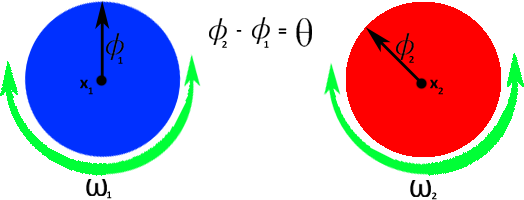
\includegraphics[width=0.75\textwidth]{pictures/rotaryDampedSpring.png}
}
\caption{\label{Fig_rotaryDampedSpring}Rotary Damped spring between two objects}
\end{center}
\end{figure}

\subsubsection{Derivation of the Impulse on a Damped Rotary Spring}
Hooke's law states:
\begin{equation*}
 F = k X
\end{equation*}

\noindent
Where X is the amount the rotary spring is displaced from its rest angle. 
\begin{equation*}
 F = k(| \phi_\text{2} -  \phi_\text{1}| - \theta)
\end{equation*}

\noindent
Impulse is a force acting over an interval of time: 
\begin{equation}
 J = k\Delta t(| \phi_\text{2} - \phi_\text{1}| - \theta) \label{eq:hooke2}
\end{equation}

\noindent
With no damping ($\zeta=0$), the above equation would be the impulse. 
With damping, an impulse to calculate the damping is needed.
The updated relative angular velocities 
between the two objects in the direction of the constraint should 
equal the old relative angular velocities multiplied by a damping value
($\gamma$).
That is:
\begin{equation}
\omega'_\text{2} -  \omega'_\text{1}=
\gamma(\omega_\text{2} -  \omega_\text{1}) \label{eq:rv_drs}
\end{equation}

\noindent
The updated angular velocities should equal:
\begin{equation*}
  \omega'_\text{1} =   \omega_\text{1} + \frac{-J}{I_\text{1}}
  \end{equation*}
  
\begin{equation*}
   \omega'_\text{2}  =  \omega_\text{2} +   \frac{J}{I_\text{2}}
  \end{equation*}

\noindent
Substituting the above equations into Eq\ref{eq:rv_drs}:

\begin{equation*}
\omega_\text{2} + \frac{J}{I_\text{2}} - \omega_\text{1} + \frac{J}{I_\text{1}}=
\gamma( \omega_\text{2}  -    \omega_\text{1})
\end{equation*}

\noindent
Factor out the impulse

\begin{equation*}
J(\frac{1}{I_\text{2}} + \frac{1}{I_\text{1}} ) + \omega_\text{2} -
\omega_\text{1}=
 \gamma( \omega_\text{2}  -    \omega_\text{1})
\end{equation*}

\noindent
Rearrange: 

\begin{equation*}
J= \frac{\omega_\text{1} - \omega_\text{2} + \gamma( \omega_\text{2} -
\omega_\text{1})}{\frac{1}{I_\text{2}} + \frac{1}{I_\text{1}}}
\end{equation*}

\noindent
Simplifying:

\begin{equation}
J= -\frac{(1-\gamma)(\omega_\text{2} - \omega_\text{1})}{\frac{1}{I_\text{2}} +
\frac{1}{I_\text{1}}} \label{eq_drs2}
\end{equation}
 
\noindent
The damping value that is used in chipmunk is:

\begin{equation*}
\gamma = e^{-\zeta(\frac{1}{I_\text{1}} + \frac{1}{I_\text{2}})t}
\end{equation*}

\noindent
Substituting the above damping value into Eq\ref{eq_drs2}:
\begin{equation}
J= \frac{(1- e^{-\zeta(\frac{1}{I_\text{1}} +
\frac{1}{I_\text{2}})t})(\omega_\text{1} -
\omega_\text{2})}{\frac{1}{I_\text{2}} + \frac{1}{I_\text{1}}} \label{eq:drag2}
\end{equation}

\noindent 
Add   Eq\ref{eq:hooke2} and Eq\ref{eq:drag2}: 
\begin{equation*}
J= k(| \phi_\text{2} - \phi_\text{1}| - \theta)\Delta t - \frac{(\omega_\text{2}
- \omega_\text{1}) (1 - e^{-\zeta (\frac{1}{I_\text{1}} + \frac{1}{I_\text{2}})
t})}{\frac{1}{I_\text{1}} + \frac{1}{I_\text{2}}}
\end{equation*}

\subsubsection{Rotary Limit Joint} \label{SecConstraintFig}
A rotary limit joint forces two bodies to be in a constant angular range to each
other
[min,max]
Figure \ref{Fig_rotaryJoint} shows an example of a rotary joint.
~\newline

%Instance Model  9 -IM9- Rotary Limit Joint
\noindent
\begin{minipage}{\textwidth}
\renewcommand*{\arraystretch}{1.5}
\begin{tabular}{| p{\colAwidth} | p{\colBwidth}|}
  \hline
  \rowcolor[gray]{0.9}
  Number& IM\refstepcounter{instnum}\theinstnum \label{IM_C_RotaryJ}\\
  \hline
  Label& \bf Rotary Limit Joint\\
  \hline
  Input& IM\ref{IM_CONSTRAINT2} , min , max \\ 
  \hline
  Output&$  J $ \\
  \hline
  Description 
&$ J= \frac{-b + \omega_\text{1} - \omega_\text{2}}{\frac{1}{I_\text{1}} +
\frac{1}{I_\text{2}}}$ \\
&\\
& b = $ \begin{cases}
\frac{k_\text{erp}}{\Delta t}(max - \phi_\text{2} - \phi_\text{1}) & \text { if
}\phi_\text{2}-\phi_\text{1}> max\\
\frac{k_\text{erp}}{\Delta t} (min - \phi_\text{2} - \phi_\text{1}) & \text { if
}\phi_\text{2}-\phi_\text{1}< min \\
  \text{0 , no impulse} & \text{otherwise}\\
  \end{cases}$ \\
  
& b = Error correction:   (DD\ref{DD_EC})\\
& min =  The minimum angle the two objects can be from each other \\
& max =  The maximum angle the two objects can be from each other \\

  \hline  
  Sources &\\
  \hline
Ref.\ By & \\
  \hline
\end{tabular}
\end{minipage}\\
~\newline

\begin{figure}[htbp]
\begin{center}
%\rotatebox{-90}
{
 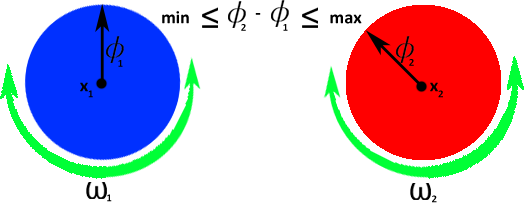
\includegraphics[width=0.75\textwidth]{pictures/rotaryJoint.png}
}
\caption{\label{Fig_rotaryJoint}Rotary Joint between two objects}
\end{center}
\end{figure}

\subsubsection{Derivation of the Impulse on a Rotary Limit Joint}
A rotary limit joint constrains the objects to
be within a certain orientation of each other. Only apply impulse if the
object's
orientations are not within [min, max] of each other. When the impulse is 
applied the relative angular velocities should be zero. That is: 

\begin{equation}
\omega'_\text{2} -  \omega'_\text{1} = 0 \label{eq:rotary_rv}
\end{equation}


\noindent 
The updated angular velocities should equal:
\begin{equation*}
 \omega'_\text{1} =   \omega_\text{1} + \frac{-J}{I_\text{1}}
  \end{equation*}
  
\begin{equation*}
  \omega'_\text{2}  =  \omega_\text{2} +   \frac{J}{I_\text{2}}
  \end{equation*}


 \noindent 
 Substituting the above equations into Eq\ref{eq:rotary_rv}:
 
\begin{equation*}
   \omega_\text{2} +   \frac{J}{I_\text{2}} -
   \omega_\text{1} + \frac{J}{I_\text{1}} = 0
 \end{equation*}
 
 \noindent 
 Factor out the impulse:
\begin{equation*}
 J(\frac{1}{I_\text{2}} + \frac{1}{I_\text{1}}) +
   \omega_\text{2}  -
   \omega_\text{1} = 0
 \end{equation*}
 
 \noindent 
 Rearranging: 
 \begin{equation*}
 J = \frac{  \omega_\text{1}  -    \omega_\text{2} }
  {\frac{1}{I_\text{2}} + \frac{1}{I_\text{1}}}
 \end{equation*}
 
 
\noindent
As mentioned in DD\ref{DD_EC} an error correction term must be added to the
angular velocity to fix potential issues with the orientation:
\begin{equation*}
 J = \frac{ -b + \omega_\text{1}  -    \omega_\text{2} }
  {\frac{1}{I_\text{2}} + \frac{1}{I_\text{1}}}
\end{equation*}


\subsubsection{Ratchet Joint} \label{SecConstraintFig}
Acts like a ratchet. Forces one body to only follow one direction of rotation
from the other body.
Figure \ref{Fig_ratchetJoint} shows an example of ratchet joint.
~\newline

%Instance Model  10 -IM10- Ratchet Joint
\noindent
\begin{minipage}{\textwidth}
\renewcommand*{\arraystretch}{1.5}
\begin{tabular}{| p{\colAwidth} | p{\colBwidth}|}
  \hline
  \rowcolor[gray]{0.9}
  Number& IM\refstepcounter{instnum}\theinstnum \label{IM_C_RatchetJ}\\
  \hline
  Label& \bf Ratchet Joint\\
  \hline
  Input& IM\ref{IM_CONSTRAINT2}, $\sigma (phase), \rho (ratchet)$\\ 
  \hline
  Output&$  J $ \\
  \hline
  Description 
&Impulse is calculated the same as \ref{IM_C_RotaryJ} except:\\

& b = $ \begin{cases}
\frac{k_\text{erp}}{\Delta t}(\theta - (\phi_\text{2}' - \phi_\text{1}')) &
\text { if } (\theta - (\phi_\text{2}' - \phi_\text{1}' ))\rho > 0 \\
\text{no impulse, } \theta = \lfloor\frac{(\phi_\text{2}'-\phi_\text{1}' -
\sigma)}{\rho}\rfloor \rho+\sigma & \text{otherwise}\\
  \end{cases}$ \\
  
& b = Error correction (DD\ref{DD_EC})\\
& $\rho$ = Ratchet. The angles which an impulse will be applied to the other
object. An impulse will be
 applied every k$\rho$ where k = 0,1,2,3..... \\
& $\sigma$ =Phase. The angle offset. An impulse will be applied every k$\rho$ +
$\sigma$ where k = 0,1,2,3..... \\
  \hline  
  Sources &\\
  \hline
Ref.\ By & \\
  \hline
\end{tabular}
\end{minipage}\\
~\newline

\begin{figure}[htbp]
\begin{center}
%\rotatebox{-90}
{
 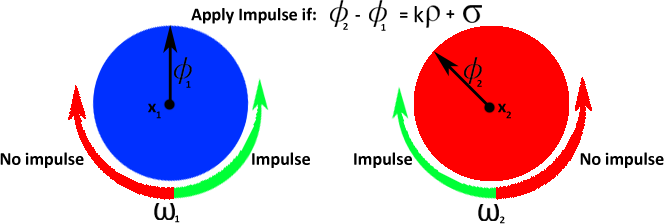
\includegraphics[width=0.75\textwidth]{pictures/ratchetJoint.png}
}
\caption{\label{Fig_ratchetJoint}Ratchet joint between two objects}
\end{center}
\end{figure}

\subsubsection{Gear Joint} \label{SecConstraintFig}
Maintains a specific angular velocity ratio between the two objects. Uses the
ratio ($\beta$) to determine how fast the opposing body will rotate.
Figure \ref{Fig_gearJoint} shows an example of a gear joint.
~\newline

%Instance Model  11 -IM11-  Gear Joint
\noindent
\begin{minipage}{\textwidth}
\renewcommand*{\arraystretch}{1.5}
\begin{tabular}{| p{\colAwidth} | p{\colBwidth}|}
  \hline
  \rowcolor[gray]{0.9}
  Number& IM\refstepcounter{instnum}\theinstnum \label{IM_C_GearJ}\\
  \hline
  Label& \bf Gear Joint\\
  \hline
  Input& IM\ref{IM_CONSTRAINT2},  $\sigma (phase), \beta(ratio)$\\ 
  \hline
  Output&$  J $ \\
  \hline
  Description &
 The updated angular velocity is calculated
differently than in IM\ref{IM_CONSTRAINT2}:\\ 

& $ \omega'_\text{1} = \omega_\text{1} + \frac{-J
}{I_\text{1}}\frac{1}{\beta}$\\
  & $   \omega'_\text{2}  =  \omega_\text{2} +   \frac{J}{I_\text{2}}$\\

&The impulse is calculated as follows:\\
&$ J= \frac{-b - \omega_\text{2}\beta +
\omega_\text{1}}{\frac{1}{I_\text{1}}\frac{1}{\beta} +
\frac{\beta}{I_\text{2}}}$ \\

& b = Error correction: $\frac{k_\text{erp}}{\Delta t}(\phi_\text{2}\beta -
\phi_\text{1} - \sigma)$ (DD\ref{DD_EC})\\
& $\beta$ = The ratio between the two angular velocities\\
&$\sigma$ = Phase.  The angle offset.\\

  \hline  
  Sources &\\
  \hline
Ref.\ By & \\
  \hline
\end{tabular}
\end{minipage}\\
~\newline

\begin{figure}[htbp]
\begin{center}
%\rotatebox{-90}
{
 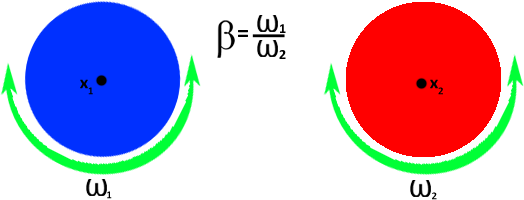
\includegraphics[width=0.75\textwidth]{pictures/gearJoint.png}
}
\caption{\label{Fig_gearJoint}Gear joint between two objects}
\end{center}
\end{figure}

\subsubsection{Derivation of the Impulse on a Gear Joint}
A gear joint maintains a specific angular velocity ratio. That is: 

\begin{equation}
\beta \omega'_\text{2} -  \omega'_\text{1} = 0 \label{eq:gear_rv}
\end{equation}

\noindent 
The updated angular velocities should equal:

\begin{equation*}
 \omega'_\text{1} =   \omega_\text{1} + \frac{-J}{I_\text{1}}\frac{1}{\beta}
  \end{equation*}
  
\begin{equation*}
  \omega'_\text{2}  =  \omega_\text{2} +   \frac{J}{I_\text{2}}
  \end{equation*}

 
 \noindent 
 Substituting the above equations into Eq\ref{eq:gear_rv}:
 
\begin{equation*}
  \beta \omega_\text{2} +   \beta \frac{J}{I_\text{2}} -
   \omega_\text{1} + \frac{J}{I_\text{1}}\frac{1}{\beta} = 0
 \end{equation*}
 
 \noindent 
 Factor out the impulse:
\begin{equation*}
 J(\frac{\beta}{I_\text{2}} + \frac{1}{I_\text{1}}\frac{1}{\beta}) +
  \beta \omega_\text{2}  -
   \omega_\text{1} = 0
 \end{equation*}
 
 \noindent 
 Rearranging: 
 \begin{equation*}
 J = \frac{  \omega_\text{1}  -   \beta  \omega_\text{2}}
  {\frac{\beta}{I_\text{2}} + \frac{1}{I_\text{1}}\frac{1}{\beta}}
 \end{equation*}
 
\noindent
As mentioned in DD\ref{DD_EC} an error correction term must be added to the
angular velocity to fix potential issues with the orientation:
 \begin{equation*}
 J = \frac{-b +  \omega_\text{1}  -   \beta  \omega_\text{2}}
  {\frac{\beta}{I_\text{2}} + \frac{1}{I_\text{1}}\frac{1}{\beta}}
 \end{equation*}
 
 
\subsubsection{Simple Motor} \label{SecConstraintFig}
 Maintains a constant angular relative velocity between the two objects. 
Figure \ref{Fig_simpleMotor} shows an example of a simple motor..
~\newline

%Instance Model 12 -IM12-  Simple Motor
\noindent
\begin{minipage}{\textwidth}
\renewcommand*{\arraystretch}{1.5}
\begin{tabular}{| p{\colAwidth} | p{\colBwidth}|}
  \hline
  \rowcolor[gray]{0.9}
  Number& IM\refstepcounter{instnum}\theinstnum \label{IM_C_SimpleM}\\
  \hline
  Label& \bf Simple Motor \\
  \hline
  Input& IM\ref{IM_CONSTRAINT2}, $\omega_\text{r}$\\ 
  \hline
  Output&$  J $ \\
  \hline
  Description 
&$ J=\frac{\omega_\text{1} - \omega_\text{2} -
\omega_\text{r}}{\frac{1}{I_\text{1}} + \frac{1}{I_\text{2}}}$ \\

& $\omega_\text{r}$= The specific angular relative velocity\\
  \hline  
  Sources &\\
  \hline
Ref.\ By & \\
  \hline
\end{tabular}
\end{minipage}\\

\begin{figure}[htbp]
\begin{center}
%\rotatebox{-90}
{
 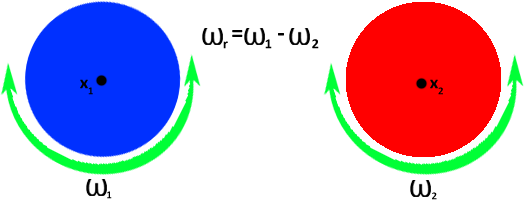
\includegraphics[width=0.75\textwidth]{pictures/simpleMotor.png}
}
\caption{\label{Fig_simpleMotor}Simple motor between two objects}
\end{center}
\end{figure}

\subsubsection{Derivation of the Impulse on a Simple Motor}
A simple motor maintains a specific angular relative velocity. That is: 

\begin{equation}
 \omega'_\text{2} -  \omega'_\text{1} = -\omega_\text{r} \label{eq:motor_rv}
\end{equation}

\noindent 
The updated angular velocities should equal:
\begin{equation*}
 \omega'_\text{1} =   \omega_\text{1} + \frac{-J}{I_\text{1}}
  \end{equation*}
  
\begin{equation*}
  \omega'_\text{2}  =  \omega_\text{2} +   \frac{J}{I_\text{2}}
  \end{equation*}

 
 \noindent 
 Substituting the above equations into Eq\ref{eq:motor_rv}:
 
\begin{equation*}
   \omega_\text{2} +   \frac{J}{I_\text{2}} -
   \omega_\text{1} + \frac{J}{I_\text{1}} = - \omega_\text{r}
 \end{equation*}
 
 \noindent 
 Factor out the impulse:
\begin{equation*}
 J(\frac{1}{I_\text{2}} + \frac{1}{I_\text{1}}) +
   \omega_\text{2}  -
   \omega_\text{1} = -\omega_\text{r}
 \end{equation*}
 
 \noindent 
 Rearranging: 
 \begin{equation*}
 J = \frac{  \omega_\text{1}  -    \omega_\text{2} - \omega_\text{r}}
  {\frac{1}{I_\text{2}} + \frac{1}{I_\text{1}}}
 \end{equation*}
 

\end{document}